\documentclass[times, utf8, diplomski]{fer}
\usepackage{booktabs}
\usepackage[final]{pdfpages}
\usepackage{hyperref}
\usepackage{amsmath}
\usepackage{bm}
\hypersetup{
    colorlinks=true,
    linkcolor=blue,
    filecolor=magenta,      
    urlcolor=cyan,
}

\begin{document}

% TODO: Navedite broj rada.
\thesisnumber{1719}

% TODO: Navedite naslov rada.
\title{Razvoj sustava globalne vizije za testiranje algoritama upravljanja bespilotnim letjelicama}

% TODO: Navedite vaše ime i prezime.
\author{Bojan Spahija}

\maketitle

% Ispis stranice s napomenom o umetanju izvornika rada. Uklonite naredbu \izvornik ako želite izbaciti tu stranicu.
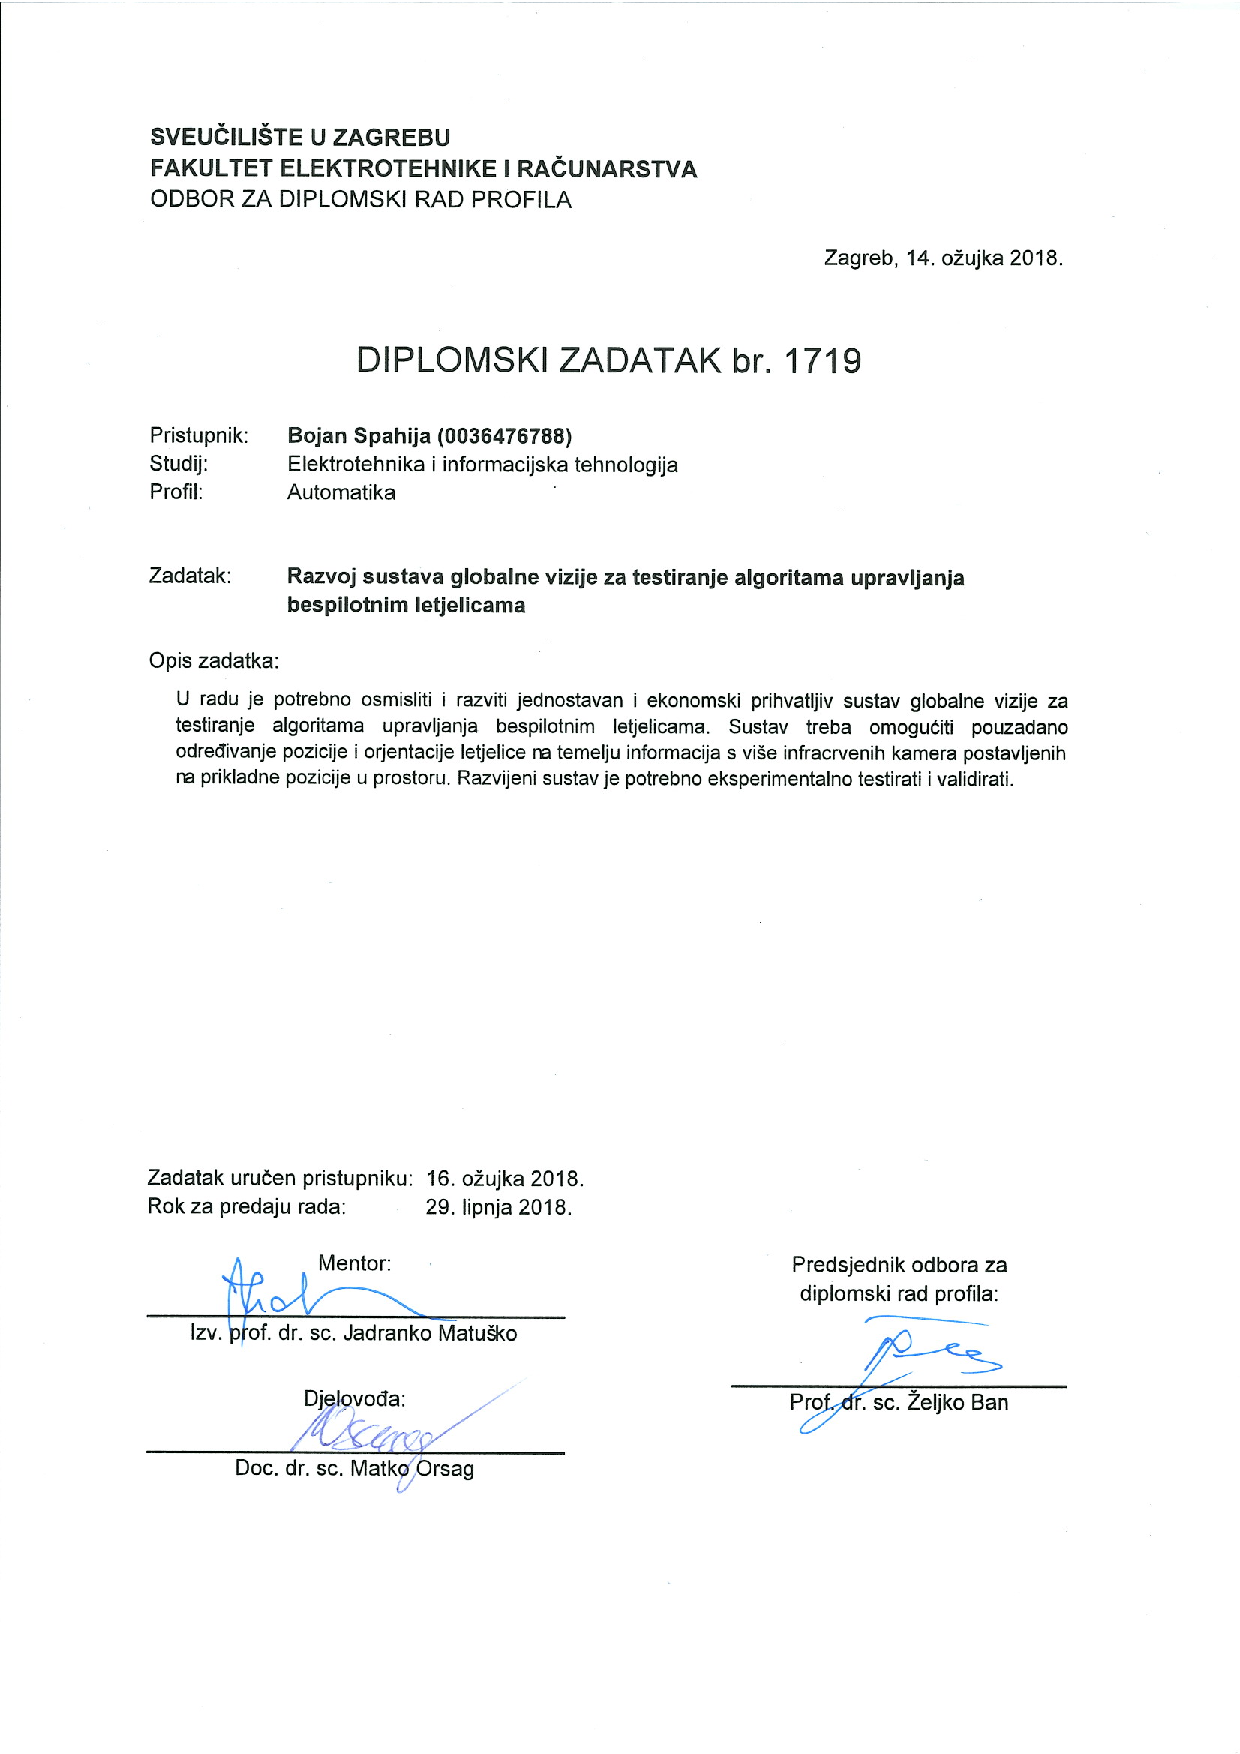
\includepdf[pages=-]{img/izvornik.pdf}

% Dodavanje zahvale ili prazne stranice. Ako ne želite dodati zahvalu, naredbu ostavite radi prazne stranice.
\zahvala{Svim ljudima dobre volje}

\tableofcontents

\listoffigures

\chapter{Uvod}
U mnogim granama industrije veliki značaj ima praćenje kretanja. Praćenje pokreta koristi se kod animacija za filmsku industriju i industriju video igara. Koristi se u vojnoj industriji za simulatore i u znanstvene svrhe za proučavanje kretanja ljudi i životinja. Zbog napretka robotike u posljednjih nekoliko godina, sve je veća potreba za preciznim praćenjem dronova i drugih robota s ciljem poboljšanja i razvoja algoritama autonomnog upravljanja.

Trenutna rješenja praćenja pokreta poput OptiTrack-a omogućuju iznimno precizno praćenje, ali vrlo su skupa. Cijene se kreću od nekoliko tisuća dolara do nekoliko desetaka tisuća dolara što nije prikladno za male firme, pojedince ili projekte za koje nije potrebna tolika preciznost. 

\chapter{Postav}
Za 3D lokalizaciju bespilotne letjelice potrebne su minimalno dvije kamere. Pomoću dvije kamere i markera koje te kamere mogu detektirati moguće je dobiti lokaciju tog markera odnosno x-y-z koordinate markera u globalnom koordinatnom sustavu. Kod upravljanja letjelicom važno je poznavati i orijentaciju letjelice (yaw). 

Upravljačke vrijednosti koje šaljemo letjelici imaju direktan utjecaj na gibanje letjelice u njezinom lokalnom koordinatnom sustavu. Da bi se poznavao utjecaj upravljačkih vrijednosti na gibanje u globalnom koordinatnom sustavu, potrebno je znati za koliko je zarotiran lokalni koordinatni sustav letjelice u odnosu na globalni koordinatni sustav (orijentacija). Kako bismo dobili informaciju o orijentaciji, potreban je specifični raspored markera koji nam omogućuje prepoznavanje orijentacije bez poznavanja orijentacije u prethodnim trenucima.

\section{Izbor kamera, IC izvora i markera}
Sustav globalne vizije mora zadovoljiti određene zahtjeve i uvjete:
\begin{itemize}
	\item Detekcija će se odvijati u zatvorenom prostoru
	\item Maksimalna udaljenost markera od kamere je oko 4m
	\item Letjelica je malih dimenzija što limitira dimenziju markera 
\end{itemize}
Zbog relativno velike udaljenosti na kojoj detekcija markera mora raditi i malih dimenzija markera, detekcija pomoću RGB kamera i markera u bojama nije pouzdana. U sustavu globalne vizije koristit će se detekcija pomoću infracrvene svijetlosti.

Infracrvena svjetlost je pogodna za detekciju na većim udaljenostima i uvjetima promjenjivog osvjetljenja. Većina materijala iz okoline reflektira vrlo malo infracrvene svjetlosti što osigurava pouzdanu detekciju infracrvenih izvora i materijala koji dobro reflektiraju infracrvenu svjetlost. Za detekciju pomoću infracrvene svjetlosti potrebni su okrugli markeri koji dobro reflektiraju infracrvenu svjetlost u svim smjerovima, kamere koje će detektirati svjetlost reflektiranu od markera i izvor infracrvene svjetlosti dovoljno velikog intenziteta i kuta zračenja da pokrije cijelo vidno polje kamere i željenu maksimalnu udaljenost markera.

\subsection{Kamera}
Testirane kamere su bile Pixy kamera sa IR-LOCK infracrvenom lećom i kamera unutar Wiimotea koja ima infracrvenu leću već ugrađenu. Obje kamere vraćaju piksele slike na kojima je detektirano infracrveno zraćenje. Valna duljina infracrvenog zraćenja koje kamere najbolje detektiraju iznosi oko 940nm. Wiimote šalje piksele od 4 najintenzivije infracrvene točke dok ih Pixy kamera može detektirati mnogo više, što u ovom slučaju ne igra ulogu zbog samo 3 potrebne točke.

Veza između Wiimotea i računala postiže se Bluetooth povezivanjem. Takva veza omogućuje veću udaljenost kamera i veću fleksibilnost kod postavljanja kamera. Direktna veza između računala i Pixy kamere može se postići mini USB kablom, a ako je nužna bežična veza potrebno je spojiti Pixy kameru na mikrokontroler koji će onda komunicirati bežično s računalom.

Također je važan vidni kut kamere jer on određuje veličinu prostora koji će se moći nadzirati. Kod Wiimote kamere horizontalni vidni kut iznosi oko 42$^{\circ}$, dok vertikalni vidni kut iznosi oko 32$^{\circ}$. Pixy kamera pokriva veće područje s horizontalnim vidnim kutem od 75$^{\circ}$ i vertikalnim vidnim kutem od 47$^{\circ}$. U segmentu vidnog polja Pixy kamera ima prednost.

Rezolucija kamere će utjecati na preciznost izračuna 3D globalnih koordinata točke. Niže rezolucije rezultiraju većim pogreškama određivanja pozicije objekata u daljini. Wiimote kamera ima vrlo malu rezoluciju od 128x96. Procesor unutar Wiimotea povećava tu rezoluciju na 1024x768 pomoću postupka analize intenziteta rubnih piksela i izračuna pozicije infracrvene točke unutar piksela (8x subpixel analysis). Ovaj postupak povećanja rezolucije kamere uvelike poboljšava preciznost detekcije usprkos korištenju jeftinih komponenata (infracrvena kamera niske rezolucije i mikroprocesor).\\
S druge strane, Pixy kamera ima ugrađenu mnogo kvalitetniju Omnivision OV9715 kameru veće rezolucije (1280x800). Pri takvoj rezoluciji, Pixy kamera radi na 25 sličica u sekundi. Kako bi se postigla veća brzina rada kamere (50 sličica u sekundi), smanjena je rezolucija na 640x400. Zbog ograničenja RAM-a koji Pixy koristi za obradu slike, rezolucija je dodatno smanjena na 320x200 piksela. Veća rezolucija Wiimotea ga čini boljim izborom zbog manje greške detekcije, a i manje cjene. Wiimote je moguće nabaviti po cijeni nižoj od \$20, dok Pixy kamera košta \$69.99.

Wiimote je bolji izbor zbog rezolucije, lakšeg povezivanja i postavljanja te niže cijene. Jedina mana mu je relativno usko vidno polje, ali taj problem se može riješiti dobrim pozicioniranjem kamera na dovoljnu udaljenost od radnog područja drona.

\subsection{Infracrveni LED izvor}
Potrebno je montirati izvor infracrvene svjetlosti uz kameru i usmjeriti ga u smjeru gledanja kamere kako bi se dobila čim bolja detekcija markera. Izvor mora biti dovoljnog intenziteta da infracrvena svjetlost bude detektirana kamerom nakon što prođe udaljenost između kamere i markera, reflektira se od markera i vrati opet do kamere. U najudaljenijoj točci radnog prostora drona ta će udaljenost biti oko 4m. Obične jeftine infracrvene diode male snage takvu udaljenost neće moći uspješno pokriti za detekciju. Dodatni problem s takvim infracrvenim diodama je relativno mali kut zračenja koji iznosi najčešće između 15$^{\circ}$ i 30$^{\circ}$. Da bi se pokrio cijeli radni prostor drona i vidno polje kamere potrebno bi bilo staviti više takvih dioda oko kamere.

Kako bi cijeli radni prostor bio dobro osvijetljen, koristiti će se infracrveni LED čipovi visoke snage od 3W (SMD LED Module) koji generira svjetlost valne duljine od 940nm. Osim veće udaljenosti koju pokriva, prednost ovakve vrste LED izvora je u širokom kutu zračenja koji iznosi 120$^{\circ}$. Tijekom testiranja ispostavilo se da 3W infracrveni LED izvori u kombinaciji s reflektirajućim markerom omogućuju detekciju markera na premaloj udaljenosti od oko 1m. Da bi se ostvarila detekcija pomoću reflektirajućeg markera potrebno bi bilo koristiti izvor jači od 10W. Zbog širokog kuta zraćenja i visoke snage, LED izvori mogu se dobro detektirati na udaljenosti do 3m pa su pogodni za markere ako se montiraju na drona.

\subsection{Marker}
Markeri koji će se nalaziti na bespilotnoj letjelici moraju biti što lakši zbog iznimno male nosivosti letjelice. Drugi zahtjev je da reflektiraju što više svjetlosti natrag prema kameri neovisno o položaju letjelice i markera. Materijali koji dobro reflektiraju infracrvenu svjetlost su neki metali (Al, Ag i Au) te oksidi metala poput SiO$_2$ i Al$_2$O$_3$. Ukoliko bi se koristili premazi ili boje koje sadrže navedene spojeve i elemente, oni bi se trebali nanjeti na lagani materijal oblika kugle koji će reflektirati svjetlost natrag kameri. U ovom slučaju važno je da marker ima oblik kugle kako bi se dio reflektirane svjetlosti, neovisno o poziciji markera i kamere, uvijek vraćao istim putem natrag prema kameri. Stiroporne kuglice zadovoljavaju zahtjeve za marker koji će biti premazan.

Druga opcija je korištenje retroreflektirajućih materijala. Retroreflektirajući materijali reflektiraju svjetlost natrag izvoru svjetlosti uz minimalno rasipanje. Zraka svjetlosti koja dolazi prema retroreflektoru je paralelna i suprotnog smjera od reflektirane zrake. Retroreflektori su najčešće male staklene ili plastične prizme. Koriste se u prometu u boji za linije na cesti i prometne znakove, kod reflektirajućih prsluka,  očiju za bicikl, itd. U slučaju odabira retroreflektora nije nužno koristiti marker oblika kugle zbog svojstva da vraća svjetlost prema izvoru neovisno o kutu upada.

Zbog infracrvenog izvora premalog intenziteta nije moguće koristiti reflektirajuće markere pa će se sam izvor koristiti kao marker. Tri izvora pričvršćena su na bespilotnu letjelicu i spojena su u paraleli na dronovu bateriju. Ovim se zadovoljavaju uvjeti detekcije, ali se skraćuje trajanje baterije zbog dodatnog napajanja LED izvora. 

\section{Pozicija kamera i markera}
Za preciznu i robusnu detekciju važno je pozicionirati kamere i markere tako da u svakom mogućem stanju letjelice unutar radnog prostora markeri budu detektirani. Robusnost je moguće postići postavljanjem viška kamera kako bi u svakom slučaju barem tri kamere vidjele markere. Također je opcija ograničenje radnog prostora letjelice tako da smo sigurni da u svim pozicijama sve kamere vide markere. 

Koriste se tri markera pozicionirana na vrhu letjelice. Markeri su postavljeni u formaciju trokuta sa jednim markerom ispred prednjeg kraja letjelice dok su druga dva markera iza stražnjeg kraja letjelice. Razmak između stražnjih markera je manji od razmaka između stražnjih i prednjeg kako bi se detektirala orijentacija letjelice.

Obje kamere moraju detektirati sva tri markera da bi se mogla odrediti pozicija i orijentacija letjelice u globalnom koordinatnom sustavu. Kamere su postavljene na pano visine 1.88m i širine 1.25m. Pozicionirane su na rubovima panoa kako bi bile što udaljenije i pokrivale što veći radni prostor. Nagib kamera prema dolje iznosi 48$^{\circ}$ (rotacija oko x-osi kamere). Kamere su zarotirane oko njihove y-osi (lijevo-desno) za 20$^{\circ}$ jedna prema drugoj kako bi se dobio što veći radni prostor. Iz poznavanja maksimalne udaljenosti detekcije koja iznosi 3m te horizontalnog i vertikalnog vidnog kuta Wiimote kamera određuje se područje unutar kojeg će obje kamere detektirati sva tri LED markera. Rubovi zone detekcije obilježeni su ljepljivom vrpcom kako bi se dron uvijek mogao precizno postaviti za eksperimente. 

\subsection{Nosač za Wiimote}
Potrebno je napraviti nosač za Wiimote kamere kako bi se dobila precizna orijentacija kamera i čvrsta veza sa objektom na kojem će kamera biti postavljena (pano). Nosač za kameru mora imati mogućnost zakreta kamere oko dvije osi, osi x i y (gore-dolje, lijevo-desno). Iz izmjerenih dimenzija Wiimotea i segmenta panoa na koji će se nosač pričvrstiti, napravljen je model modularnog nosač u Solidworksu i isprintan pomoću 3D printera. Nosač se sastoji od 3 dijela:

\begin{enumerate}
	\item Držač Wiimotea
	\item Učvršćivač za pano
	\item Segment za vezu između fiksiranih dijelova 
\end{enumerate}

Veza između držača Wiimotea i segmenta za vezu ostvarena je preko ploha koje sjedaju jedne između drugih. Dok su plohe poravnate još postoji mjesta za micanje pa je moguće postaviti željenu rotaciju Wiimotea oko x-osi (gore-dolje). Kada je postavljeni željeni kut rotacije, umetanjem M3 vijka kroz rupu u plohama i njegovim zatezanjem pomoću matice učvršćuje se veza i osigurava željena rotacija.

Veza između dijela učvršćenog na pano i segmenta za povezivanje ostvarena je preko cilindra na koji se postavlja segment za povezivanje. Segment za povezivanje se može slobodno rotirati oko vertikalne osi (lijevo-desno). Kad se postavi željeni zakret Wiimotea, veza se učvršćuje pomoću M3 matice i vijka. 

\subsection{Radni prostor}
Iz pozicija i orijentacija kamera, poznatog vidnog kuta i maksimalne udaljenosti na kojoj Wiimoteovi detektiraju infracrveni LED marker računa se prostor unutar kojeg je kamera u mogućnosti detektirati marker. Taj postupak se radi za obje kamere. Presjek prostora detekcije prve i druge kamere je radni prostor. Ako dron ostane unutar tog prostora njegova pozicija i orijentacija će biti dobivene iz sustava globalne vizije pa je važno postaviti ograničenja radnog prostora u algoritme upravljanja dronom kako on ne bi izašao tog prostora.

Zbog ručnog postavljanja zakreta kamera koje unosi greške od nekoliko stupnjeva i loše detekcije markera na rubnim dijelovima vidnog polja kamera, određivanje rubova radnog prostora izvršeno je eksperimentalno.  

\chapter{Komunikacija}
Oba Wiimotea se povezuju bežično preko Bluetooth veze sa osobnim računalom. Računalo mora na neki način dohvatiti bitne informacije iz kamera, iz njih izračunati poziciju i orijentaciju drona u prostoru te na kraju objaviti izračunate vrijednosti kako bi se one mogle dohvatiti od strane upravljačkog algoritma. Za preciznu detekciju i pouzdano upravljanje važno je da su mjerenja kamera sinkronizirana te da je poznata frekvencija izračuna i objave pozicije drona. Frekvencija kojom Wiimote šalje podatke iznosi 100Hz. Za upravljanje po poziciji takva brzina je nepotrebna pa će se uzimati podaci frekvencijom od 20Hz. Robotski operacijski sustav će se koristiti za uspostavu komunikacije jer zadovoljava sve uvjete i omogućuje precizno i brzo izvršavanje više Python ili C++ skripti za dohvat, obradu i objavu informacija.
 
\section{ROS - Robot Operating System}
Velika složenost zadataka koji se postavljaju pred moderne robote zahtijeva korištenje programske infrastrukture koja omogućuje efikasno povezivanje nezavisno razvijenih podsustava u jedinstveni sustav koji može omogućiti autonomno djelovanje robota. Robotski operacijski sustav (ROS) pruža okolinu za razvoj modularne upravljačke programske podrške, komunikacijsku infrastrukturu koja povezuje programske komponente, te otvorenu biblioteku implementiranih algoritama. U posljednjih 5 godina, ROS je postao de facto standard za upravljanje robotima unutar akademske zajednice, te se njegova primjena širi i na industriju.

ROS nam u ovom projektu olakšava komunikaciju između nezavisnih Python skripti preko publish/subscribe sistema. Također nam omogućuje lako snimanje podataka koje objavljuje neka od skripti i ponovno objavljivanje tih podataka kasnije.

ROS čvor (node) je proces koji vrši izračune i obradu informacija. Više čvorova međusobno komunicira preko tema (topics). Kontrolni sustav će obično imati mnogo čvorova koji vrše manje specijalizirane zadatke. Prednost ovakvog sustava s mnogo čvorova je otpornost na greške jer se greške i rušenja u programu svode na rušenja pojedinog čvora, a ne cijelog sustava. Složenost koda je također smanjena zbog modularnosti te je testiranje sustava jednostavnije.

ROS teme su imenovani kanali kroz koje se odvija anonimna komunikacija između čvorova. Čvorovi se mogu pretplatiti na bilo koju od prisutnih tema pomoću Subscriber objekta ili mogu objavljivati podatke u zadanoj temi pomoću Publisher objekta. Tema može imati više pretplaćenih čvorova (subscribers) i objavljujućih čvorova (publishers). Vrsta teme ovisi o tipu poruke koja je objavljena na nju. Pretplaćeni čvorovi moraju dohvaćati tip podataka koji odgovara vrsti teme.

\section{ROS - Implementacija}
Sustav za globalnu viziju će se sastojati od tri čvora. Po čvor za primanje podataka sa svakog Wiimotea te čvor za obradu dobivenih mjerenja Wiimotea i objavu izračunate pozicije i orijentacije. Čvor za komunikaciju s Wiimoteom već postoji pa je skinut s interneta. Koristi se "wiimote" paket iz skupa paketa "joystick\textunderscore drivers" (\url{https://github.com/ros-drivers/joystick_drivers}). Ovaj paket se ne može koristiti za uspostavu komunikacije s više Wiimoteova. Ako se povežu oba Wiimotea pomoću njega, čvorovi će objavljivati mjerenja na istu temu i time brisati objave jedan drugom pa nije moguće dohvaćati mjerenja. Problem je riješen dodavanjem "id" parametra. Prilikom pokretanja čvora i povezivanja s Wiimoteom zadajemo identifikacijski broj koji mijenja naziv tema tako da dopiše parametar "id" na kraj postojećeg naziva teme. Novi čvor koji se koristi pokreće se Python skriptom wiimote\textunderscore node.py i nalazi se u paketu "wiimote".

Ovime se postiže da umjesto jedne teme naziva /wiimote/state dobijemo dvije teme: /wiimote/state1 i /wiimote/state2. Sada je lako dohvatiti mjerenja oba Wiimotea i možemo spojiti više Wiimoteova ako će biti potrebno.

Čvor za obradu mjerenja pretplaćeni je na /wiimote/state1 i /wiimote/state2 teme koje objavljuju modificirani čvorovi za dohvat podataka s Wiimoteova. Tip poruke koja se dohvaća je wiimote/State.msg tipa. Ovaj tip poruke sadrži mnoge nepotrebne podatke poput stanja tipki na Wiimoteu i njegovu akceleraciju pa je u funkciji dohvata potrebno izolirati samo važne podatke. Jedini potrebni podaci su pikseli na kojima su detektirani infracrveni izvori. Wiimote vraća taj podatak u obliku liste od 4 elementa, a svaki element je wiimote/IrSourceInfo.msg tipa podatka koji u sebi sadrži x i y detektiranog piksela. U nastavku je prikazan kod funkcije dohvata piksela.

\vspace{5mm}  

Nakon što uspješno primi detektirane piksele od obje kamere, čvor za obradu izvršava izračun pozicije i orijentacije, koji će biti opisan kasnije u radu, te objavljuje dobivenu poziciju i orijentaciju na temu /drone\textunderscore position u obliku tipa podatka geometry\textunderscore msgs/Quaternion.msg. Quaternion tip poruke se koristi za objavu jer sadrži 4 varijable float64 tipa, a objavljena poruka nema veze sa stvarnim kvaternionima. Varijable "x", "y" i "z" predstavljaju poziciju u globalnom koordinatnom sustavu dok varijabla "w" predstavlja orijentaciju drona, to jest zakret njegovog lokalnog koordinatnog sustava u odnosu na globalni oko z-osi (yaw). Čvor koji ima funkciju upravljačkog algoritma drona će čitati iz teme /drone\textunderscore position što će omogućiti da se zatvori upravljačka petlja po poziciji i orijentaciji.

\chapter{Izračun pozicije i orijentacije}
Nakon što su kamere postavljene i usmjerene, markeri postavljeni na dronu i komunikacija uspostavljena, slijedi problem izračuna globalne pozicije točke iz poznatih piksela na kamerama. Svaki Wiimote objavljuje piksel na kojem je detektirao infracrveni marker. Taj piksel je zapisan u obliku (x,y) gdje x predstavlja stupac u kojem je piksel s prvim stupcem na lijevom kraju slike, a zadnjim stupcem (1024. stupac) na desnom kraju slike, dok y predstavlja redak s prvim retkom na dnu slike, a zadnjim na vrhu (768. red). Potrebno je iz para piksela (x$_1$, y$_1$) za prvi Wiimote i (x$_2$, y$_2$) za drugi Wiimote izračunati poziciju te točke u globalnim koordinatama (x$_G$, y$_G$, z$_G$). Prvi postupak kojim se to pokušalo postići je pomoću geometrije i poznatih parametara kamere.

\section{Geometrijski postupak}
U ovom postupku koristiti će se "pinhole" model kamere za opis matematičkog odnosa koordinata točke u tri dimenzije i njezine projekcije na slikovnu ravninu. Ovaj model opisuje kameru točkom i ne uzima u obzir utjecaje leće poput iskrivljenja slike i zamućenje objekata koji nisu u fokusu. Točnost pinhole modela opada udaljavanjem od središta slike prema rubovima zbog povećanja iskrivljenja slike.

\subsection{Formiranje slike u pinhole kameri}
Sve zrake svjetlosti koje ulaze u točkasti model kamere i formiraju sliku prolaze kroz optički centar. Slikovna ravnina kamere je pomaknuta iza optičkog centra za udaljenost koja odgovara žarišnoj duljini kamere \textit{f}. Dobivena slika na slikovnoj ravnini je izokrenuta pa se ona dodatno invertira kako bi dobili krajnju sliku. Inverzija slikovne ravnine odgovara projekciji točke na ravninu koja je postavljena ispred optičkog centra za žarišnu duljinu kamere. Središte 3-D koordinatnog sustava kamere (X, Y, Z) postavljeno je u optički centar \textit{O}. Koordinatni sustav slikovne ravnine (x', y') postavljen je u točki gdje Z-os koordinatnog sustava kamere siječe slikovnu ravninu.

Sve jednadžbe vezane uz projekciju slijede iz sličnosti trokuta formiranih stvarnom točkom \textit{p}(x, y, z) u koordinatnom sustavu kamere, projekcijom te točke u koordinatnom sustavu slikovne ravnine i optičkim centrom.

\begin{equation}
\frac{x'}{x} = \frac{f}{z}
\label{eq:projekcija1}
\end{equation}

\begin{equation}
\frac{y'}{y} = \frac{f}{z}
\label{eq:projekcija2}
\end{equation}

\subsection{Određivanje točke pravcima}
Iz jednadžbi \ref{eq:projekcija1} i \ref{eq:projekcija2} vidi se da je potrebno poznavati žarišnu duljinu kamere \textit{f}, projiciranu točku (x', y') te barem jedan vektor (x, y ili z) točke \textit{p} ako želimo odrediti koordinatu na kojoj se točka nalazi. Treba riješiti problem određivanja tri parametra iz dvije jednadžbe. Premda je poznato da su točka, njezina projekcija i optički centar na istom pravcu, moguće je izračunati taj pravac. Žarišna udaljenost Wiimote kamere iznosi $f=1280$. Poznat je broj piksela od sredine slike prema rubovima pa se računa maksimalni vertikalni i horizontalni kut pod kojim pravac može ulaziti u kameru.

\begin{equation}
\alpha_{max} = arctg\bigg(\frac{x'_{max}}{f}\bigg)
\label{eq:alpha1}
\end{equation}

\begin{equation}
\beta_{max} = arctg\bigg(\frac{y'_{max}}{f}\bigg)
\label{eq:beta1}
\end{equation}

\vspace{5mm}

Iz rezolucije Wiimote kamere koja iznosi 1024x768 dolazimo do vrijednosti:

\begin{equation}
x'_{max} = \frac{1024}{2} = 512 \qquad\text{i}\qquad y'_{max} = \frac{768}{2} = 384
\label{eq:pix_max}
\end{equation}

\vspace{5mm}

Nakon uvrštavanja vrijednosti \ref{eq:pix_max} u jednadžbe \ref{eq:alpha1} i \ref{eq:beta1} dolazimo do vrijednosti maksimalnog vertikalnog i horizontalnog kuta pravca koje iznose $\alpha_{max} = 21.8^{\circ} \quad\text{i}\quad \beta_{max} = 16.7^{\circ}$ . Kako bi se saznalo za koliko svaki piksel po x' osi slike i po y' osi slike mijenja $\alpha$ i $\beta$ kut pravca, maksimalne vrijednosti kuteva dijele se s $x'_{max}$ odnosno $y'_{max}$:

\begin{equation}
\Delta\alpha = \frac{\alpha_{max}}{x'_{max}} = 0.0426^{\circ}
\label{eq:d_alpha}
\end{equation}  

\begin{equation}
\Delta\beta = \frac{\beta_{max}}{y'_{max}} = 0.0435^{\circ}
\label{eq:d_beta}
\end{equation}

\vspace{5mm}

Jednadžbe \ref{eq:d_alpha} i \ref{eq:d_beta} vrijede u idealnom slučaju kada ne dolazi do iskrivljenja slike na rubovima. Poznato je za koliko stupnjeva svaki piksel po x' osi i y' osi mijenja usmjerenje pravca od pravca koji izlazi ravno iz kamere (po Z-osi koordinatnog sustava kamere). Slijede jednadžbe za izračun kuteva zakreta iz poznatog piksela (x', y'):

\begin{equation}
\alpha = (512 - x')\Delta\alpha
\label{eq:alpha}
\end{equation}

\begin{equation}
\beta = (-384 + y')\Delta\beta
\label{eq:beta}
\end{equation}

\vspace{5mm}

Iz poznatih kuteva slijedi izračun jediničnog vektora u koordinatnom sustavu kamere \textit{O} koji pokazuje u smjeru pravca na kojem leži točka \textit{p}:

\begin{align}
x &= sin(\alpha)cos(\beta) \\
y &= sin(\beta) \\
z &= cos(\alpha)cos(\beta)
\end{align}

\vspace{5mm}

Sljedeći korak je transformacija vektora koji pokazuje na točku iz lokalnog koordinatnog sustava kamere (X, Y, Z) u globalni koordinatni sustav ($X_G$, $Y_G$, $Z_G$). Prvo će se izvršiti rotacija tog vektora pa onda translacija. Iz poznate pozicije kamere i orijentacije njenog lokalnog koordinatnog sustava računamo translacijsku i rotacijsku matricu. Koristi se Z-Y-X rotacijska matrica, što znači da se lokalni koordinatni sustav prvo rotira za kut $\psi$ oko svoje Z-osi, onda rotira za kut $\theta$ oko svoje novo pozicionirane Y-osi, te na kraju rotira za kut $\phi$ oko X-osi. Za svaku od ovih rotacija, koristi se pripadna rotacijska matrica te se množe u ispravnom poretku $R_{Z}(\psi)R_{Y}(\theta)R_{X}(\phi)$.

\begin{equation}
	\begin{bmatrix}
		X_G \\
		Y_G \\
		Z_G
	\end{bmatrix}
	= R_{Z}(\psi)R_{Y}(\theta)R_{X}(\phi)\cdot
	\begin{bmatrix}
		X \\
		Y \\
		Z 
	\end{bmatrix}
	+ \begin{bmatrix}
		X_{trans} \\
		Y_{trans} \\
		Z_{trans} 
	\end{bmatrix}
\end{equation}

\begin{equation}
	R_{Z}(\psi) = 
	\begin{bmatrix}
		cos(\psi) & -sin(\psi) & 0 \\
		sin(\psi) & cos(\psi) & 0 \\
		0 & 0 & 1 \\
	\end{bmatrix}
\end{equation}

\begin{equation}
	R_{Y}(\theta) = 
	\begin{bmatrix}
		cos(\theta) & 0 & sin(\theta) \\
		0 & 1 & 0 \\
		-sin(\theta) & 0 & cos(\theta) \\
	\end{bmatrix}
\end{equation}

\begin{equation}
	R_{X}(\phi) = 
	\begin{bmatrix}
		1 & 0 & 0 \\
		0 & cos(\phi) & -sin(\phi) \\
		0 & sin(\phi) & cos(\phi) \\
	\end{bmatrix}
\end{equation}

\vspace{5mm}

Nakon što je završena transformacija vektora u globalni koordinatni sustav, poznat nam je pravac na kojem leži točka. Da bi se mogla odrediti točna pozicija te točke na pravcu potrebna je druga kamera. Kada se isti postupak određivanja pravca na kojem leži točka obavi i za drugu kameru, traži se presjek pravca iz prve i iz druge kamere u idealnom slučaju. Zbog ručnog postavljanja kuteva zakreta kamera, diskretizacije piksela i nesavršenosti kamera, slučaj da se pravci sijeku je skoro nemoguć. Zato se traže točke na oba pravca gdje su pravci najbliži jedan drugom.

Za izračun najbližih točki na pravcima, kreće se od parametarske jednadžbe pravca koja glasi:

\begin{equation}
\bm{l} = \bm{p_0} + \bm{d}\cdot t
\label{eq:pravac}
\end{equation}

\vspace{5mm}

U jednadžbi \ref{eq:pravac} $\bm{p_0}$ je neka poznata točka na pravcu, $\bm{d}$ je vektor smjera pravca, a $t$ je skalar koji određuje pomak točke od $\bm{p_0}$ po pravcu u smjeru $\bm{d}$.

Ako su poznate jednadžbe dvaju pravaca: 
\begin{equation}
\bm{l_1} = \bm{p_1} + \bm{d_1}\cdot t_1 \qquad\text{i}\qquad \bm{l_2} = \bm{p_2} + \bm{d_2}\cdot t_2
\label{eq:pravci}
\end{equation}

Pravac koji povezuje najbliže točke pravca $\bm{l_1}$ i $\bm{l_2}$ mora biti okomit na oba pravca. Vektorskim produktom vektora smjera pravaca $\bm{d_1}$ i $\bm{d_2}$ dobiva se vektor tog okomitog pravca, $\bm{n}$.

\begin{equation}
\bm{n} = \bm{d_1} \times \bm{d_2}
\end{equation}

Najbliža točka na pravcu $\bm{l_1}$ pravcu $\bm{l_2}$ je na presjecištu pravca $\bm{l_1}$ i ravnine koja se dobi širenjem pravca $\bm{l_2}$ u smjeru $\bm{n}$. Jednadžba te ravnine može se izraziti kao skup točaka $\bm{p}$ za koje vrijedi:

\begin{equation}
(\bm{p} - \bm{p_0})\cdot\bm{n_R} = 0
\label{eq:ravnina}
\end{equation}

U jednadžbi \ref{eq:ravnina}, $\bm{p_0}$ označava točku koja se nalazi na ravnini, a $\bm{n_R}$ označava vektor normale te ravnine. Ravnina koja nam je potrebna za pronaći najbližu točku na pravcu $\bm{l_1}$, sadrži točku $\bm{p_2}$, a jednadžba njene normale $\bm{n_2}$ dobit će se vektorskim produktom vektora smjera pravca $\bm{d_2}$ i $\bm{n}$.

\begin{equation}
\bm{n_2} = \bm{d_2} \times \bm{n} = \bm{d_2} \times (\bm{d_1} \times \bm{d_2})
\end{equation}

Jednadžba ravnine koja sadrži pravac $\bm{l_2}$ i najbližu točku pravca $\bm{l_1}$ tada glasi:

\begin{equation}
(\bm{p} - \bm{p_2})\cdot \bm{n_2} = 0
\label{eq:ravnina2}
\end{equation}

Kako bi se dobila točka u kojoj pravac $\bm{l_1}$ sječe ovu ravninu, u jednadžbu \ref{eq:ravnina2} uvrštava se jednadžba za pravac $\bm{l_1}$.

\begin{equation}
(\bm{p_1} + \bm{d_1}\cdot t_1 - \bm{p_2})\cdot \bm{n_2} = 0
\label{eq:presjek}
\end{equation}

Potrebno je dobiti $t_1$ za koji vrijedi jednadžba \ref{eq:presjek}. Rješavanjem jednadžbe za $t_1$ dobije se:

\begin{equation}
t_1 = \frac{(\bm{p_2} - \bm{p_1})\cdot \bm{n_2}}{\bm{d_1}\cdot\bm{n_2}}
\end{equation}

\vspace{5mm}

Ponavljanjem postupka za pravac $\bm{l_2}$ dobit će se $t_2$. Uvrštavanjem izračunatih $t_1$ i $t_2$ u jednadžbe pravaca $\bm{l_1}$ i $\bm{l_2}$ (jednadžba \ref{eq:pravci}) dobit će se najbliže točke na pravcima, $\bm{c_1}$ i $\bm{c_2}$.

\begin{equation}
\bm{c_1} = \bm{p_1} + \frac{(\bm{p_2} - \bm{p_1})\cdot \bm{n_2}}{\bm{d_1}\cdot\bm{n_2}}\bm{d_1}
\end{equation}

\begin{equation}
\bm{c_2} = \bm{p_2} + \frac{(\bm{p_1} - \bm{p_2})\cdot \bm{n_1}}{\bm{d_2}\cdot\bm{n_1}}\bm{d_2}
\end{equation}

\vspace{5mm}
 
Opisani postupak pronalaska najbližih točaka dvaju pravaca koristi se u ROS čvoru zaduženom za obradu informacija pristiglih od kamera i objavu pozicije i orijentacije drona. Ovaj čvor pokreće se Python skriptom \textit{wii\textunderscore detection.py}. Funkcija \textit{line\textunderscore distance} zadužena je za pronalazak točaka i njihove udaljenosti.

Svi koraci opisani u ovom odlomku izvršavaju se unutar \textit{wii\textunderscore detection} čvora. Prvi korak je učitavanje mjerenja oba Wiimotea. Iz dobivenih piksela vrši se izračun pravca na kojem je marker u lokalnom koordinatnom sustavu kamere. Izračunati pravci se prebacuju iz lokalnih koordinata u globalne. Od svake kamere se dobiva od nula do tri pravca. Potrebno je upariti ispravne pravce prve i druge kamere kako bi se dobile dobre točke. Svaki pravac prve kamere se uspoređuje sa pravcima druge kamere i traži se najmanja udaljenost. Uzima se pravac druge kamere kojem je pravac prve kamere najbliži za izračun pozicije markera prema kojem ti pravci gledaju. Ukoliko nije niti jedan marker detektiran, objavljuje se pozicija drona $x=-1.0$, $y=-1.0$, $z=-1.0$. Ukoliko je detektiran samo jedan marker, objavljuje se pozicija tog markera. Kod dva ili tri markera dodatno se računa pozicija centra drona te njegova orijentacija.
 
\section{Postupak pomoću neuronske mreže}

Drugi postupak koji se koristio za određivanje pozicije markera iz para piksela dobivenih od kamera bio je postupak pomoću neuronske mreže. Kod geometrijskog postupka nisu se uzeli u obzir intrinzični parametri kamera te su kamere morale biti vrlo precizno postavljene kako ne bi došlo do promašivanja pravaca i krive detekcije. Cilj ovog postupka je naučiti jednostavnu unaprijednu (\textit{engl.} feedforward) neuronsku mrežu odgovarajućih dimenzija kako preslikati parove piksela (x$_1$, y$_1$) za prvi Wiimote i (x$_2$, y$_2$) za drugi Wiimote u globalne koordinate točke (x$_G$, y$_G$, z$_G$). Dobro naučena neuronska mreža bi trebala moći precizno modelirati to preslikavanje, čak ako postoje neki nepoznati utjecaji i nelinearnosti. Mana ovog postupka je da se ne smije mijenjati nagib i pozicija kamera jer se učenje vrši s točno određenim položajem kamera.

\subsection{Osnove neuronskih mreža}

Ideja umjetnih neuronskih mreža proizašla je iz načina funkcioniranja bioloških neuronskih mreža. Biološki neuron, kao osnovna gradivna jedinica biološke neuronske mreže, prima i obrađuje informacije od drugih neurona i/ili od osjetilnih organa. Može se pojednostavljeno prikazati kao stanica sastavljena od tijela (soma), mnoštva dendrita i aksona. Mali razmak između završetka aksona prethodnoga neurona i dendrita sljedećeg neurona naziva se sinapsa. Akson jednoga neurona formira sinaptičke veze s mnoštvom drugih neurona. Impulsi, koji se generiraju u tijelu neurona, putuju kroz akson do sinapsi. Ovisno o učinkovitosti svakog pojedinačnog sinaptičkoga prijenosa, signali različitog intenziteta dolaze do dendrita. Učinkovitost sinaptičkoga prijenosa kroz neku sinapsu ovisi o njezinom elektrokemijskom stanju, koje je rezultat prethodnih sinaptičkih prijenosa kroz nju. Signali se od sinapsi dendritima proslijeđuju do tijela neurona, gdje se prikupljaju i obrađuju. Ovi signali mogu za tijelo neurona biti pobuđujući ili smirujući. Matematički gledano, pobuđujući i smirujući signali imaju suprotan predznak. Ako je njihova kumulativna vrijednost tijekom kratkog vremenskog intervala veća od praga osjetljivosti neurona, tijelo neurona generira impulse (tzv. aktivacijske potencijale) koji se šalju duž aksona prema drugim neuronima, a ako je manja, neuron ostaje nepobuđen i ne generira impulse.

\vspace{5mm}

\textit{Perceptron} je jednostavan model umjetnog neurona koji vrši slične operacije kao i biološki neuron. Sinaptička je operacija predstavljena množenjem svakog ulaznog signala $x_i$ s težinskim koeficijentom $w_i$. Otežani se ulazni signali zbrajaju i njihov se zbroj uspoređuje s pragom osjetljivosti neurona $w_{n+1}$. Ako je zbroj otežanih signala veći od praga osjetljivosti neurona, nelinearna aktivacijska funkcija $\psi$ generira izlazni signal neurona $y$ iznosa jedan, a ako je manji, izlaz neurona je nula.

U radu će se koristiti statički model neurona. Njegov izlaz ovisi isključivo o trenutnim vrijednostima ulaznih signala i težinskim koeficijentima. Matematički se može opisati sljedećim izrazima:

\begin{equation}
v(t) = \sum_{i=1}^{n}w_i(t)\cdot x_i(t) - w_{n+1}
\end{equation}

\begin{equation}
y(t) = \psi(v)
\end{equation}

gdje je:

$\bm{X_u}(t) = [x_1(t),...,x_n(t)]^T$ - vektor ulaznih signala neurona;

$\bm{W_s}(t) = [w_1(t),...,w_n(t)]^T$ - vektor sinaptičkih težinskih koeficijenata;

$w_{n+1}$ - prag osjetljivosti neurona;

$v(t)$ - izlaz operacije konfluencije;

$\psi(v)$ - nelinearna aktivacijska funkcija;

$y(t)$ - izlaz neurona

\vspace{5mm}

Većina neuronskih mreža zahtijeva učenje, to jest primjenu algoritama koji podešavaju iznose sinaptičkih težinskih koeficijenata. Ciljevi učenja mreže ovise o njezinoj primjeni, pa tako i izbor odgovarajućeg algoritma učenja. Iako je razvijen veliki broj raznih
algoritama učenja neuronskih mreža, moguće ih je po načinu učenja mreže podijeliti na algoritme učenja temeljene na pogrešci, algoritme učenja temeljene na izlazu mreže i algoritme učenja s ojačanjem. U radu će biti korišteni algoritmi učenja temeljeni na pogrešci.

\textit{Algoritmi učenja temeljeni na pogrešci} često se nazivaju i algoritmi s “učiteljem” jer zahtijevaju vanjski referentni signal (učitelj) s kojim uspoređuju dobiveni odziv neuronske mreže generirajući signal pogreške. Na temelju signala pogreške algoritam učenja mijenja sinaptičke težinske koeficijente neuronske mreže s ciljem poboljšanja njezina vladanja, to jest smanjenja pogreške. Ovi se algoritmi mogu primijeniti samo ako je unaprijed poznato željeno vladanje neuronske mreže, to jest podaci na osnovi kojih se mreža uči moraju sadržavati parove vrijednosti ulazno-izlaznih signala.

\subsection{Implementacija neuronske mreže}



\chapter{Rezultati}

\chapter{Zaključak}
Zaključak.

\bibliography{literatura}
\bibliographystyle{fer}

\begin{sazetak}
U mnogim granama industrije veliki značaj ima praćenje kretanja. Prisutna rješenja poput OptiTrack-a osiguravaju precizno praćenje, ali su iznimno skupa. Cilj rada je razvoj jednostavnog i ekonomski prihvatljivog sustava globalne vizije za praćenje pozicije i orijentacije bespilotnih letjelica. Sustav se sastoji od dvije infracrvene kamere i tri infracrvena markera postavljena na dronu. Za određivanje pozicije markera u globalnom koordinatnom sustavu potrebne su minimalno dvije kamere. Minimalno tri markera potrebna su kako bi se mogla izračunati orijentacija drona uz njegovu poziciju. Kao kamera se koristi Wiimote koji sadrži jednostavnu infracrvenu kameru, a markeri su infracrveni LED izvori velike snage (3W). Komunikacija između Wiimoteova i osobnog računala ostvarena je pomoću Bluetootha i ROS čvora. Iz poznatih pozicija kamera i dobivenih točaka od svakog Wiimotea, osobno računalo računa globalnu poziciju svake točke te iz tih pozicija računa orijentaciju i poziciju drona. Orijentacija i pozicija se objavljuju preko ROS-a kako bi se mogli dohvatiti od strane upravljačkog algoritma. 

\kljucnerijeci{praćenje pokreta, sustav vizije, dronovi, infracrvene kamere, Wiimote, markeri, pozicija, orijentacija, ROS}
\end{sazetak}
\newpage

% TODO: Navedite naslov na engleskom jeziku.
\engtitle{Development of a Global Vision System for Testing of Control Systems for Unmanned Aerial Vehicles}
\begin{abstract}
Motion tracking systems are of great importance in many industries. Current solutions like OptiTrack ensure precise tracking, but are very expensive. The goal of the project is the development of a simple and economically acceptable global vision system for drone position and orientation tracking. The system is made of two static infrared cameras and three infrared markers placed on the drone. To determine the position of the markers in the global coordinate system a minimum of two cameras is needed. At least three markers are needed in order to calculate the orientation of the drone. The camera used in the project is the IR camera inside a Wiimote and the markers used are high power IR LED sources (3W). The communication between the Wiimotes and the PC is realized using Bluetooth and a ROS node for each Wiimote. From the known Wiimote positions and the points detected by the Wiimotes, the PC calculates the global position of each point and then uses those positions to calculate the orientation and position of the drone. Orientation and position are published to a ROS topic, so that the control algorithm can acquire them.

\keywords{motion tracking, vision system, drones, infrared cameras, Wiimote, markers, position, orientation, ROS}
\end{abstract}

\end{document}
